\section{Project management}
There is a consensus amongst the team members that our adaptation of Scrum has worked well as a project management framework. Combining this with our adaptation of Extreme Programming has led to a very agile and responsive development process. To ensure productivity preventative measures were taken early on in the process. A monetary penalty was instated for arriving late to meetings or not delivering work on time. The money accumulated from this was spent on a team building evening for the team members. Every Wednesday a team member would be responsible for bringing snacks and making sure the team took regular breaks. Both of these ensure higher productivity and well-being within the team.

\subsection{Working with the customer}
The team tried to have meetings with the customer once a week. This worked well and the team felt that it was a good thing that the customer participated to such an extent. Initially we had some trouble with the customer not meeting deadlines set together with the team. These deadlines affected the teams research early on in the project. The customer was to set the team in contact with people at Sintef that could have information about hardware solutions. As this requirement was dropped early on it did not have a huge effect. However, while in China the team received an email detailing the Cossmic api described in section~\ref{sec:cossmicapi}. We feel that having this information early on might have made the system as a whole easier to develop in the future. As the information was received so late in development, the team and customer agreed on not implementing it, but rather write some documentation on how it could be used in further development.

\subsection{Changing roles}
\label{sec:unbalancedWorkload}
In the beginning of the project, the team distributed roles with different responsibilities. A project leader, a deputy project leader, a scrum master, a development responsible, a test responsible and a report responsible. Almost halfway through the project it became clear that the scrum master at the time, Per Øyvind, was also the one with the most Android experience. This resulted in a lot of extra work on the scrum master, while the deputy project leader had no extra responsibilities at all. Therefore, the team reflected over the project roles and the distribution, and this resulted in a change of roles. The team then decided that Lars Erik, which previously was our deputy project leader, was the best fit to be the new Scrum master. After this change the team's best Android resource could focus entirely on developing the app and helping others. The team was very satisfied with this decision, and efficiency and productivity increased after the change in roles.

It was also discussed whether the position `Project leader' actually was necessary, as it conflicted with one of the principles in Scrum. The team decided that the position was necessary as the project leader and Scrum master simply would share the Scrum master's traditional tasks between them. The main difference would be that the project leader would handle the administrative tasks, such as booking rooms for meetings and work sessions, and handle customer relations, while the Scrum master would handle the project administrative tasks. These tasks include moderating of the Scrum meetings, adding tasks to the backlog and Yodiz, and generate burn down charts.

\subsection{Choice of development methods}

The team chose to use scrum together with extreme programming. This process and why these were chosen is described in section \ref{sec:scrumDevProcess} and~\ref{sec:adapExtremeProgr}. Even though Scrum is well known, many team members had different expectations to how the framework would be implemented in the project.

Each team member spent a significant amount of time getting up to date with the Android platform and the front-end architecture of Android apps. In retrospect, more time should have been spent getting all group members up to date and practicing Android programming together in the beginning of the project. One of the team members had some experience with Android before and ended up spending a lot of time teaching and explaining to the other team members. If this had been organized in a way, for instance by holding a course in the beginning, some of the time spent on this could have been saved. 

\subsection{Underestimation of workload}
A prevalent risk to any project is the failure to acknowledge the cost of tasks in the project and the improper allocation of resources that follows such an error. This can also lead to a false sense of what a team can achieve in a given time frame. 

The team experienced this risk to have the biggest negative impact on our work flow. Even though it did not have a detrimental effect on the sprint end result, it was the most occurring risk, which added up to be very time consuming. The main reason for this issue was the lack of experience with many of the tasks, but also that we initially did not consider who the tasks were assigned to which turned out to play an important role in the equation. Learning from previous mistakes, the team started looking at previous sprint backlogs to help estimate the cost of work packages.

\subsection{Choice of Scrum tool}
\label{sec:choiceScrumTool}
As the team did not have daily meetings, a good scrum tool was needed to keep track of progress. Having bad experiences with scrum tools from previous project, the team decided to spend some time to research the candidates. After deciding on Yodiz, the team was confident it had chosen the best option available free of charge (including student licenses). This might still be true, but using Yodiz still proved to be somewhat of a annoyance for the team members. The fact of the matter is that a digital scrum tool is very hard to design in an intuitive fashion. Combine this with poor support for simultaneous editing and you end up with a system that causes a lot of problems. However, Yodiz was the only tool that covered all the requirements set by the team, and despite its obvious flaws, it did its job. Ideally, the team would have liked to have a meeting room with a scrum board so the use of such an extensive scrum tool could be avoid altogether. At the end of the project the team started using a scrum board in the the meeting room used on workday meetings. This should have been done earlier in the project.

\subsection{Improper use of Yodiz}
\label{sec:improperScrum}
As mentioned in section~\ref{sec:scrumtool}, the team used a lot of time on
deciding on which Scrum tool to use for the project management. Although our
choice fell on Yodiz, the team was in lack of any previous experience with the
tool, and despite the team's efforts to get acquainted with the tool, a
misunderstanding arose and was not discovered until the end of the second
sprint.

The misunderstanding, displayed in figure~\ref{fig:wrongUse}, was that the team
assumed one could add multiple individuals as responsible on a particular task,
while Yodiz' functionality only assigned the time spent to the individual that
either created the task or was assigned as owner of the task.

As a result, it appeared as if only singular individuals performed the tasks,
even though the entire team in reality was participating, which was also
reflected in the burn down charts and the generated Gantt diagram. 

To sort out this issue, the team went through old meeting reports and time sheets
to figure out which members of the team that had actually participated on the
particular task, and added new tasks and the time spent to the members that at
the time had not recorded this information.%, as shown in figure~\ref{fig:addsTasks}.

This issue was unfortunate, but not insurmountable, and also not a critical
issue for the overall progress of the project.

\begin{figure}[H]
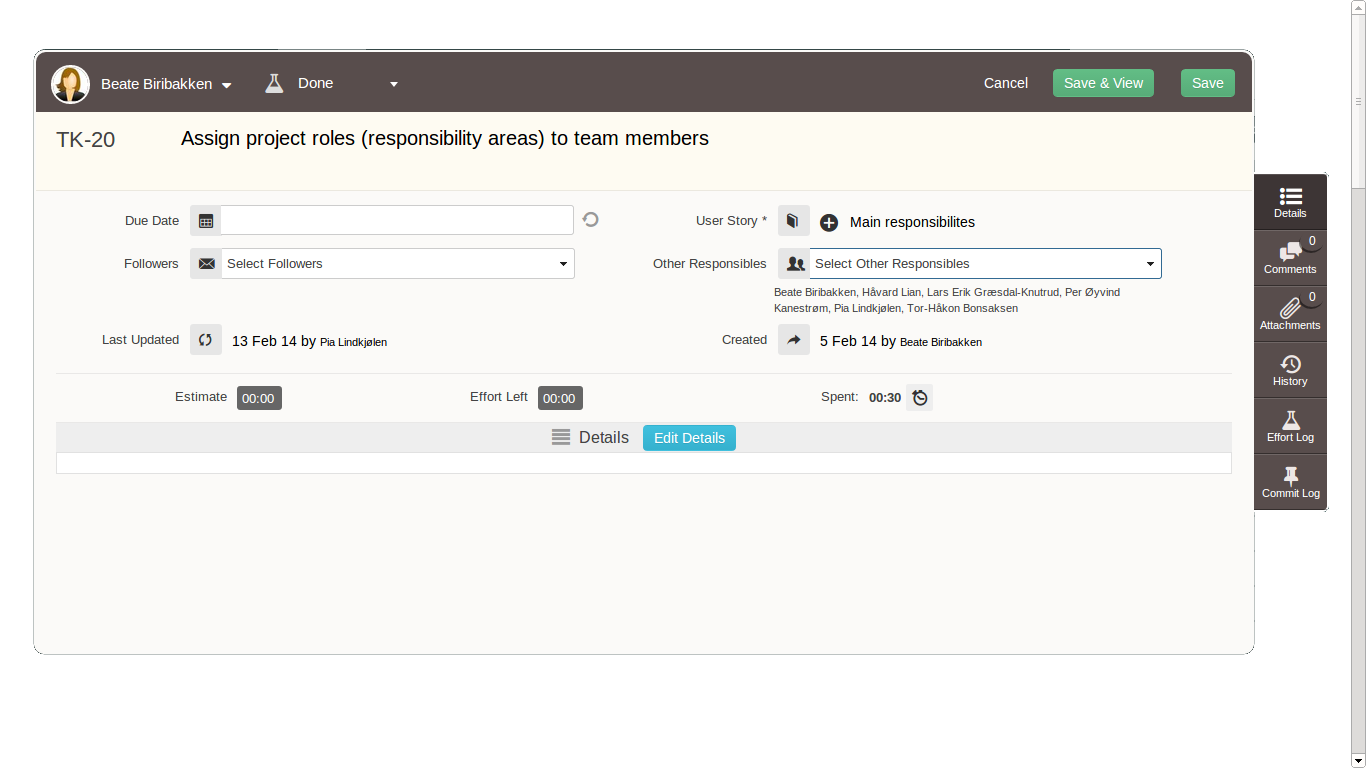
\includegraphics[width=\textwidth, clip, trim=1cm 2cm 4cm 1cm]{ch/retrospect/fig/wrongUse.png}
\caption{Example screenshot to illustrate improper use of Yodiz.}
\label{fig:wrongUse}
\end{figure}
